\chapter{Data and Methods} \label{chap:data}

In this section, we broadly explain the structure of Facebook's advertisement ecosystem, the data we gather from the system, and the techniques we use to analyze it.

\section{Facebook's Advertisement Ecosystem} \label{sec:fb_ad_eco}

% LATER: for thesis draft, explain the scale of how many people are affected by these ads and how important all of it is to Facebook.

As the world's largest social network\footnote{\url{https://www.weforum.org/agenda/2017/03/most-popular-social-networks-mapped/}}, Facebook's targeted advertising system allows marketers and businesses to target ads to its users by their demographic attributes, location, interests and internet behaviors. Prior to launching an ad, Facebook is also able to report how many people would fit the criteria and view the campaign -- which it refers to as the \textit{reach estimate}.

The ability of the platform to a) simultaneously target users by both their demographic and behavioral attributes; and b) to provide reach estimates prior to actually launching the ads, makes it a useful tool for understanding the characteristics of a population. It also makes it a powerful tool for understanding what Facebook \textit{thinks} the characteristics of a population are.

We are able to use the system for very specific queries such as ``the number of women between the ages of 25 and 29 interested in online shopping" or ``the number of African-American men managing small business pages on Facebook", and then compare the given reach estimates across demographic groups -- all without ever launching an ad.

On a more general level, Facebook categorizes its ad targeting toolkit into three major categories\footnote{\url{https://www.facebook.com/business/products/ads/ad-targeting}}:

\begin{enumerate}
\item \textbf{Core Audiences:} Here, Facebook allows marketers to choose the features of the population they want to target. These features range from demographic variables such as gender and relationship status to interests in things such as anime movies or hip hop music. Section \ref{subsec:targeting_options} discusses the available options in detail.

\item \textbf{Custom Audiences:} This feature allows marketers to upload a list of personally identifiable information (PII), which is then matched to accounts on Facebook for targeted advertising.

\item \textbf{Lookalike Audiences:} In lookalike targeting, Facebook is able to expand on an initial list of people provided by the marketer (for instance, through a PII list or through a prior ad campaign). Facebook builds the target audience by looking for people with similar interests and features to the ones provided.
\end{enumerate}

We primarily choose to focus on core audiences, as our goal is to identify biases present in the features provided to advertisers.

\subsection{Available Targeting Options} \label{subsec:targeting_options}

\begin{figure}

\centering
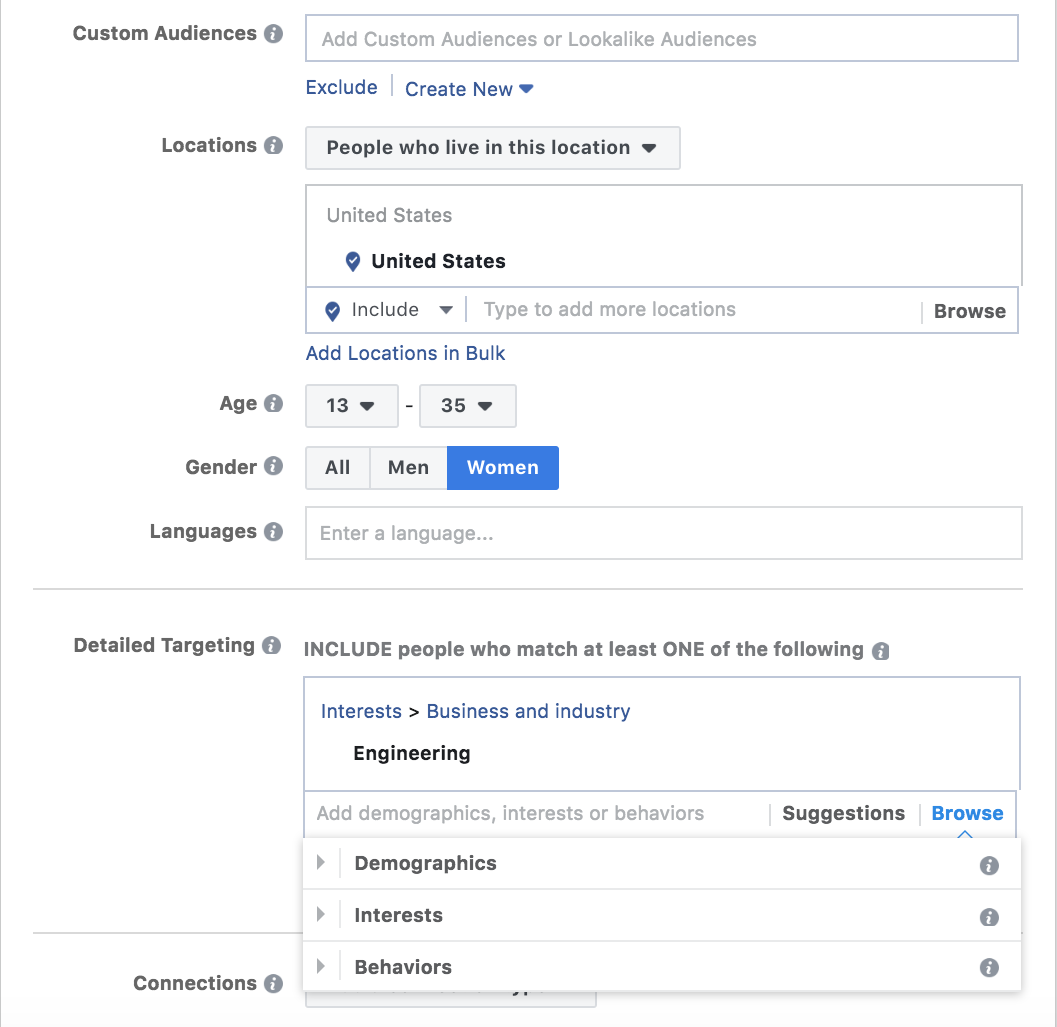
\includegraphics[width=.8\textwidth]{ad_interface}
\caption{Screenshot of Facebook's Ads Manager interface showing some of the major functionalities available. Geographical location, age and gender have been specified. An elaborate list of targeting options are available through the cascading drop-down menus under ``Detailed Targeting". Here, the category ``Engineering" has been selected.}
\label{fig:ad_interface}

\end{figure}

Figure \ref{fig:ad_interface} shows the structure of Facebook's \textit{Ads Manager} page, where marketers can construct audiences for advertisement campaigns. We see that the interface provides the option to target by location, age, gender, language and a wide array of options under the ``Detailed Targeting" section.

For location based targeting, Facebook provides the option to target countries, regions comprising multiple countries (e.g. Asia or the European Economic Area), regions within countries such as provinces or states, cities, ZIP codes, as well as congressional districts in the United States. It also allows radius targeting by dropping a pin at a particular address and specifying a target radius as small as 1 kilometer around it. For all these options, advertisers are able to target people who either live in the area, have recently traveled there, are currently traveling, or all of the above.

In selecting age, the interface permits arbitrary age ranges with the minimum and maximum age options. Since the social network's minimum allowed joining age is 13, the platform doesn't allow targeting pre-teens.

Under detailed targeting, the platform classifies interests into three broad categories: demographics, interests and behaviors. Targeting features such as education level, relationship status and employment are grouped under demographics. The interests category contains features related to what people might be interested in, such as professions, entertainment choices, or health interests, among others. Behaviors mostly contains features where Facebook collaborates with external data-brokers to identify user behaviors on the internet. It also contains categories such as users' device usage, shopping behaviors, or their expat status. Facebook plans to permanently discontinue collaborating with external data brokers in August 2018 but other categories under behaviors will stay.

It is also important to note that the list of these targetable features is not static by any means. It is subject to moderation if the users report a feature in the list as inappropriate. As an example, this public moderation practice has previously led to Facebook renaming the ethnic affinity feature \cite{propublica_fb_ethnic_affinity_again} and removing problematic anti-semitic ad categories that were automatically indexed by the ad system \cite{propublica_jew_hater_study}.


In addition to the features characterized under these three categories, Facebook also automatically indexes other interests across the platform which advertisers can search by inputting free text. Many of these features have been observed to be directly related to pages on the social network and are explained in the Ads Manager as targeting ``people who have expressed an interest in" or ``like pages related to" the particular feature.
% To briefly characterize the kinds of features that are grouped together, Table \ref{tab:top_10_attrs} shows the most popular interests and behaviors for Facebook users in the US.

Further, the interface permits splitting the detailed targeting option into three sub-fields, allowing for different mechanisms of adding targeting features:

\begin{enumerate}
\item \textbf{Include}: The default field as shown in Figure \ref{fig:ad_interface} shows the include option. Features added to this field are combined together with a logical OR operation to match the audience. Each subsequent feature added here acts to expand the audience.

\item \textbf{Narrow}: Unlike the include option, features are combined in this field with a logical AND operation. Features added to this field serve to refine and narrow the audience.

\item \textbf{Exclude}: People who match features listed under the exclude section are explicitly excluded from the ad's audience.
% Features added to this field explicitly exclude certain members of the current targeted population.
\end{enumerate}

Using the three functions, marketers are able to construct arbitrarily complex and niche audiences. For instance, a targeting combination such as:
$$(\text{electrical engineering} \lor \text{software engineering}) \land \text{mathematics} \land \neg \text{design}$$
% people who are interested in electrical engineering OR software engineering AND mathematics and NOT in design, is a perfectly valid combination.
is perfectly possible and permitted with the current targeting mechanism.

Throughout the process of tweaking the audience by selecting different targeting options, Facebook reports the number of people accessible with the current selection. This is shown under \textit{Potential Reach} in the Ads Manager and is shown in Figure \ref{fig:reach}. These reach estimate form the foundation of our study and are the primary measurements we take from the online ads network.

\begin{figure}

\centering
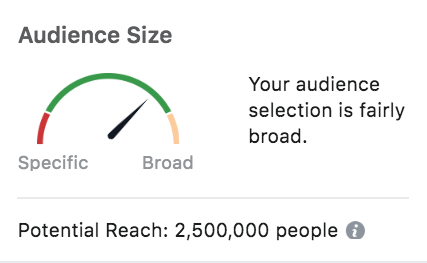
\includegraphics[width=.5\textwidth]{reach}
\caption{Size of targetable population (reach estimate) with the targeting options selected in Figure \ref{fig:ad_interface} i.e. women living in the United States, between the ages of 13 and 35, who are interesting in engineering.}
\label{fig:reach}

\end{figure}

\subsection{The Marketing API} \label{subsec:marketing_api}
To encourage developers to programmatically create and manage ad campaigns, Facebook has provided public Application Programming Interfaces (APIs). By making a developer account on the platform and setting up an application with appropriate permissions, we are also able to leverage these APIs for research purposes. In particular, we utilize the Marketing API to specify combinations of targeting features, demographic attributes, and geographical locations -- in return for the reach estimates for these combinations.

We also take advantage of the Targeting Search API -- the same API that is used to search Facebook's database of features when an advertiser inputs free text. By sending an empty string query, we are able to retrieve all features grouped under interests and behaviors from the platform.

Facebook also provides convenient Software Developer Kits (SDKs) for different programming languages for abstractions in access to the APIs. We make use of the Facebook Business SDK for Python\footnote{\url{https://github.com/facebook/facebook-python-business-sdk}} to make queries to the Marketing and Targeting Search APIs.

\subsection{Data Collected} \label{subsec:data_collected}
We collect both demographic and advertisement related estimates from the Marketing API. Demographically, we choose to focus on gender and ethnicity; while for the advertisement estimates, we query the API for the interest each demographic group shows in the ad-targeting features. We limit our estimates to the United States as it is a high internet penetration country, and also the only region where Facebook explicitly infers ethnicity -- or ``Multicultural Affinity" as the Ads Manager calls it.

\textbf{Demographics:} For gender, we ask Facebook for the number of men and women in the U.S. For ethnicity, we query for the number of White, Asian, Hispanic and African Americans in the country. Since Facebook doesn't have an explicit White ethnicity attribute, we obtain this estimate by excluding all other ethnic groups recorded by the platform.

\textbf{Targeting Features:} Once we have the list of targeting attributes from the Targeting Search API -- 323 interests and 264 behaviors, we are able to iterate over them and ask the Marketing API for a) the number of people interested in the attribute; and b) the number of people from each demographic group interested in the attribute. The latter estimate is made with a logical AND (the narrow option) in the API.

\section{Quality of Facebook's Estimates} \label{sec:fb_quality}
Since our study focuses on Facebook's ad-targeting features and their associations along different demographic dimensions, it is imperative that Facebook's estimates for these demographic variables are reliable. Gender and age are self-reported on the social network, while ethnicity (available only in the United States) is an inferred feature. Errors might arise either due to faulty self-reporting or due to problems in Facebook's inference.

To investigate the quality of demographic estimates from Facebook's API, we compare the gender and ethnicity estimates to ground truth data from the American Community Survey's 2016 1-year estimates. The American Community Survey (ACS) is a survey administered by the United States Census Bureau in addition to the decennial census to annually update housing and demographic statistics \cite{acs2017info}. We use the developer API provided by ACS to query for ground truth data.

As of the time of this writing, the Ads Manager reports that 240 million people who live in the United States are targetable with Facebook ads. To understand the scale of this penetration, we stratify this estimate by each state and observe what fraction of the population in each state is targetable. Figure \ref{fig:rep_map} shows the fraction of population in each state that is targetable with Facebook's targeted ads. We find that the lowest penetration is in New Jersey with 58.13\% of the population being targetable. The average penetration over all states is 69.45\%. This helps illustrate the scale of the platform in a country like the U.S. where a large fraction of the population is reachable and can be studied with advertisement data.

% ==== map figure ====
\begin{figure}
\centering
\includegraphics[width=\textwidth]{representation}
\caption{State level penetration of Facebook advertisements in the United States. In every state, at least half of the population is reachable with targeted advertising.}
\label{fig:rep_map}
\end{figure}
% ====

% === correlation figures ===
% === for smaller figure widths, this would put images side by side ===
\begin{figure}
    \centering
    \subfloat[Men. $\rho=0.996 \;(p < 10^{-20})$; $R^2=0.992$.]{{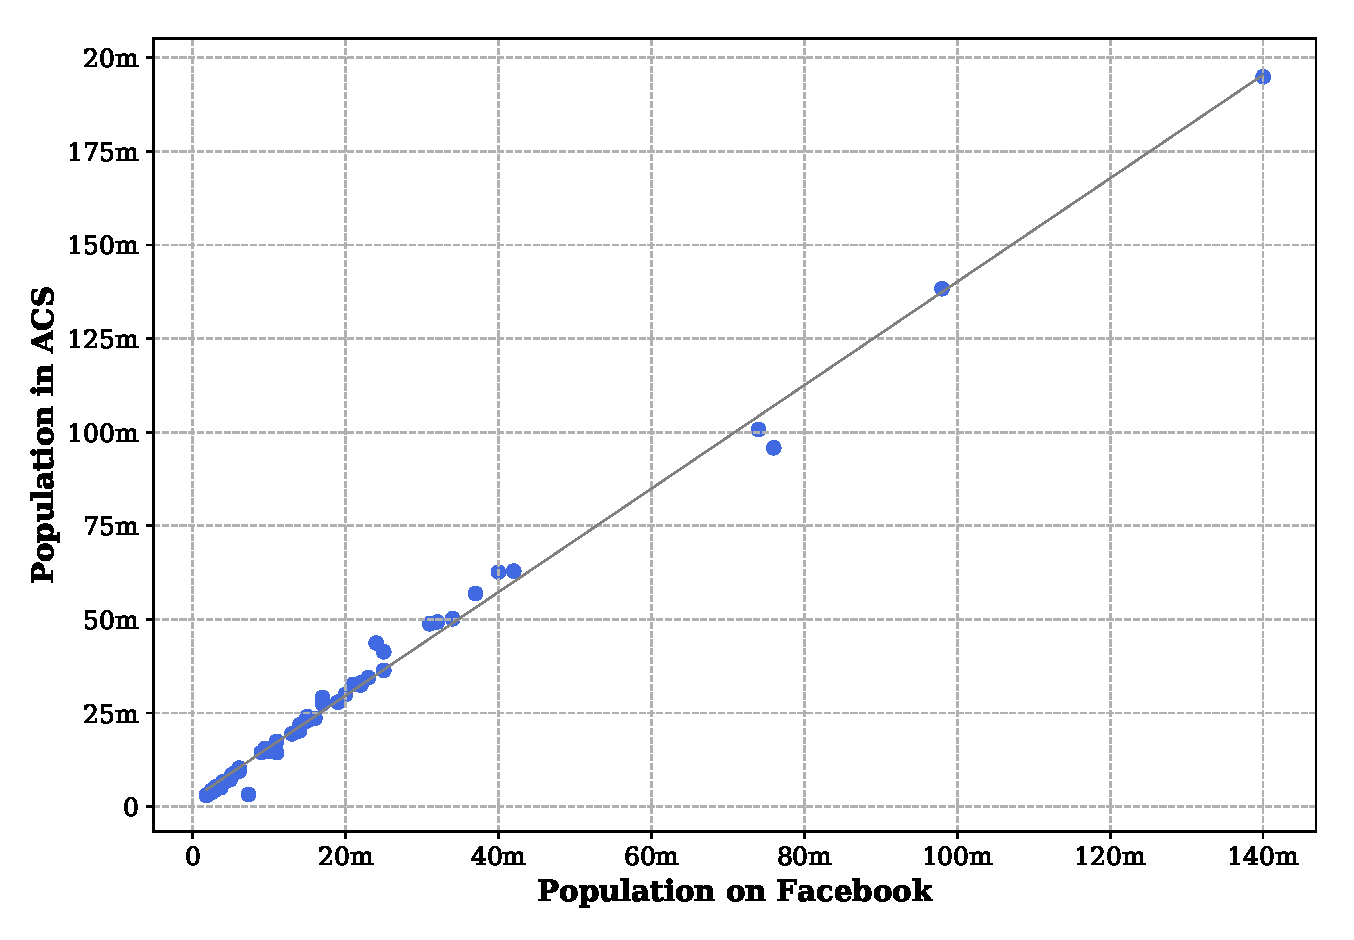
\includegraphics[width=.75\textwidth]{men_corr} }}
    \qquad
    \subfloat[African Americans. $\rho=0.983 \;(p < 10^{-20})$; $R^2=0.966$.]{{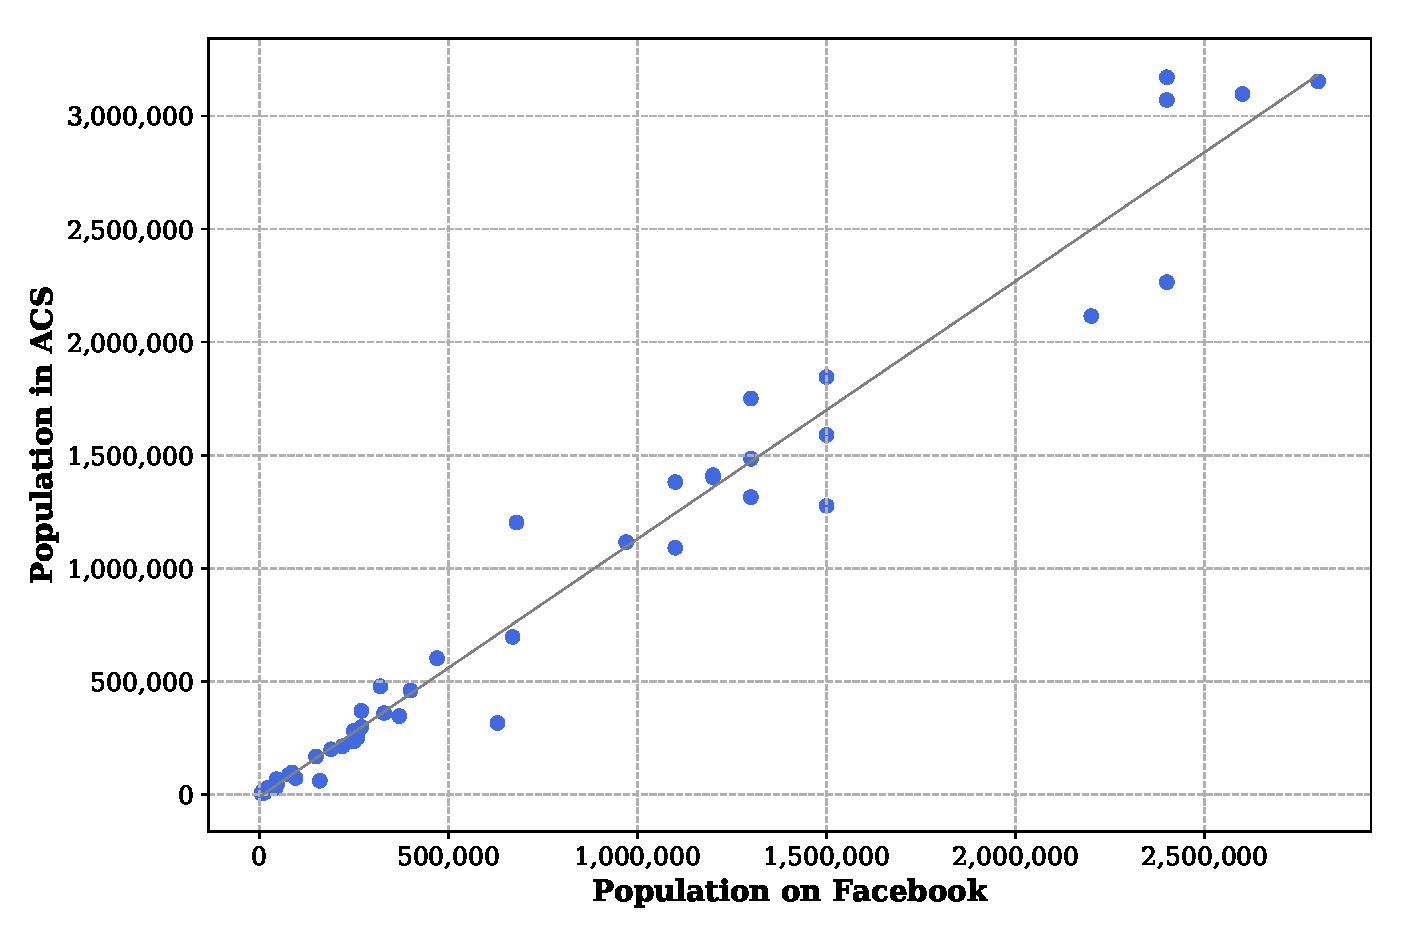
\includegraphics[width=.75\textwidth]{black_corr} }}

    \caption{Gender and ethnicity estimate comparisons from Facebook with ground truth data from the American Community Survey (ACS). Above: Comparison for gender estimates; the number of men in each state is shown. Below: Comparison for ethnicity estimates; the number of African Americans in each state is shown. The grey lines show a linear regression model fit to the estimates from Facebook. The correlation coefficient $\rho$, and the coefficient of determination $R^2$ for the linear model have been reported.}
    \label{fig:corrs}
\end{figure}
% ====

To ensure the quality of gender and ethnicity estimates, we compare Facebook's estimates against ground truth, state-level data obtained from the developer API provided by ACS\footnote{\url{https://www.census.gov/data/developers/data-sets.html}}. Querying over different states serves the dual purpose of a) having multiple measurements of the same variables, and b) establishing that our approaches are extensible to smaller geographies. Figure \ref{fig:corrs} shows how the state-level estimates for gender and ethnicity correlate across Facebook and ACS. It can be seen that Facebook is able to estimate both variables extremely well, and most variance can be explained with a simple linear model. Table \ref{tab:corrs} shows the comparison for all possible values of gender and ethnicity in Facebook's API.

These results demonstrate that even though not everyone is on Facebook or targetable with its online ads, there are no significant skews in the predictions that the ad platform makes for demographic variables. This gives us confidence that analyses built on top of these estimates are reliable and not spurious due to poor quality estimates.

\begin{table}
\centering
\begin{tabular}{c | c | c } 
\toprule
\textbf{Variable} & \textbf{Value} & \textbf{$\rho$}\\
 \hline
\textbf{Gender} & Male & 0.9963\\
& Female & 0.9979\\
 \hline
 \textbf{Ethnicity} & White & 0.9667\\
 & African American & 0.9833\\
 & Asian American & 0.9934\\
 & Hispanic & 0.9842\\
\end{tabular}
\caption{Correlations of Facebook's state-level gender and ethnicity estimates with American Community Survey's (ACS) ground truth data. $p < 10^{-20}$ for all rows.}
\label{tab:corrs}
\end{table}


\section{Methods for Analysis} \label{sec:methods}
Once we have collected data from the marketing API and ensured that Facebook's demographic estimates corroborate with real-world data, we begin evaluating which targeting features have the highest affiliations with which subgroups of the population.

% In this section, we operationalize the biases investigate our data for.

To quantify how likely it is for a particular demographic group to be inferred interested in a targeting feature, we define the notion of \textit{interest affinity}. Simply put, the interest affinity captures whether a group is more or less interested than the general population in a targetable feature according to Facebook. Since these inferences are done by Facebook and we only access data from a blackbox, we essentially capture whether the ad might have associated ad interests with demographic groups. More formally, we define the affinity for a demographic group $d$ towards a targetable feature $f$ as

\begin{equation}
\text{affinity}_g(d, f) = \frac{n_g(d, f)}{n_g(d)} - \frac{n_g(f)}{N_g},
\label{eq:aff}
\end{equation}

where $n_g(d)$ and $n_g(f)$ are the reach estimates (i.e. number of people targetable) by specifying demographic $d$ and feature $f$ alone. $n_g(d, f)$ refers to the intersection of populations targetable with $d$ and $f$. Because of the nature of the ad ecosystem, a geographical location of the audience must always be specified, which is what the $g$ in the subscript refers to. Consequently, $N_g$ is the total population in region $g$ according to Facebook. All these estimates are obtained with the data collection process described in Section \ref{subsec:data_collected}.

A large positive value would indicate that members of demographic $d$ are considered much more likely by the ad platform to be interested in feature $f$, as compared to the general population in region $g$. Analogously, a large negative value would mean Facebook does not associate group $d$ with the feature $f$ and some other subgroup of the population in $g$ is more highly interested.

For brevity, we shall hereon refer to the first term in Equation \ref{eq:aff} as the \textit{penetration} of feature $f$ within demographic $d$ i.e.

\begin{equation}
\text{penetration}_g(d, f) = \frac{n_g(d, f)}{n_g(d)}
\label{eq:pen}
\end{equation}

It simply characterizes what fraction of a demographic $d$ is considered interested in feature $f$ by Facebook.

Naturally, for two groups $d_1$ and $d_2$ that have a large difference in their affinity (or alternatively, penetration) for a particular feature $f$, Facebook has a very different understanding of their interest in $f$. As a result, a higher fraction of the group with the larger affinity would end up seeing content related to $f$. We refer to the difference in affinity for two groups as their \textit{disparity} on targetable feature $f$

\begin{align*}
\text{disparity}_g(d_1, d_2, f) &= \text{penetration}_g(d_1, f) - \text{penetration}_g(d_2, f)\\
&= \frac{n_g(d_1, f)}{n_g(d_1)} - \frac{n_g(d_2, f)}{n_g(d_2)} \addtocounter{equation}{1}\tag{\theequation}
\label{eq:disparity}
\end{align*}

Having a notion of disparity between two demographics in terms of a targetable feature $f$ allows us to investigate what differences Facebook believes these groups have. It also allows us to be more rigorous by performing significance testing on the disparity. For a set of targeting features $F$ and a feature $f^* \in F$ with positive value of the disparity statistic $T = \text{disparity}_g(d_1, d_2, f^*)$, we are able to compute the p-value with a maximum likelihood estimate as

\begin{align*}
p &= \Pr[\; \text{disparity}_g(d_1, d_2, f) \geq T \;]\\[.3em]
&= \frac{\big|\{f \in F \; | \; \text{disparity}_g(d_1, d_2, f) \geq T\}\big|}{|F|} \addtocounter{equation}{1}\tag{\theequation}
\label{eq:p_val_positive}
\end{align*}

In our situation, $F$ is the set of all features that we have gathered from Facebook's APIs. Similarly, for negative values of the disparity statistic, we look towards more extreme negative values to compute the p-value,

\begin{align*}
p &= \Pr[\; \text{disparity}_g(d_1, d_2, f) \leq T \;]\\[.3em]
&= \frac{\big|\{f \in F \; | \; \text{disparity}_g(d_1, d_2, f) \leq T\}\big|}{|F|} \addtocounter{equation}{1}\tag{\theequation}
\label{eq:p_val_negative}
\end{align*}

This simple but useful way of significance testing gives us a clear idea of the strength of any difference in feature disparities. Using this framework, we are able to answer questions like whether there are significant differences between men and women in Facebook's inference of professional features such as engineering; or what kind of industries the ad platform associates most with African Americans. Moreover, we are able to do this without launching any malicious or harmful ads and only through the reach estimates provided in the Ads Manager.